% (meta)
% Exercise contributed by chinwei
% label: ch8

\Exercise{
\label{ex:weightnorm}
This question is about weight normalization. We consider the following parameterization of a weight vector $\vw$:
$$\vw := \gamma\frac{\vu}{||\vu||}$$
where $\gamma$ is scalar parameter controlling the magnitude and $\vu$ is a vector controlling the direction of $\vw$.
\begin{enumerate}
\item Consider one layer of a neural network, and omit the bias parameter. 
To carry out batch normalization, one normally standardizes the preactivation and performs elementwise scale and shift $\hat{y}=\gamma\cdot\frac{y-\mu_y}{\sigma_y}+\beta$ where $y=\vu^\top\vx$. 
Assume the data $\vx$ (a random vector) is whitened ($\Var(\vx)=\mI$) and centered at $0$  ($\E[\vx]=\mathbf{0}$). 
Show that $\hat{y}=\vw^\top\vx+\beta$. 
\item Show that the gradient of a loss function $L(\vu,\gamma,\beta)$ with respect to $\vu$ can be written in the form $\nabla_\vu L=s\mW^\perp\nabla_\vw L$ for some $s$, where $\mW^\perp=\left(\mI-\frac{\vu\vu^\top}{||\vu||^2}\right)$.
Note that \footnote{As a side note: $\mW^\perp$ is an orthogonal complement that projects the gradient away from the direction of $\vw$, which is usually (empirically) close to a dominant eigenvector of the covariance of the gradient. This helps to condition the landscape of the objective that we want to optimize.} $\mW^\perp\vu=\mathbf{0}$.
\item Figure~\ref{fig:weightnormgrowingnorm} shows the norm of $\vu$ as a function of number of updates made to a two-layer MLP using gradient descent. 
Different curves correspond to models trained with different log-learning rate. 
Explain why (1) the norm is increasing, and (2) why larger learning rate corresponds to faster growth. 
(Hint: Use the Pythagorean theorem and the fact that 
$\mW^\perp \vu = 0$ from question 4.2).
\end{enumerate}
\begin{figure}[h]
\centering
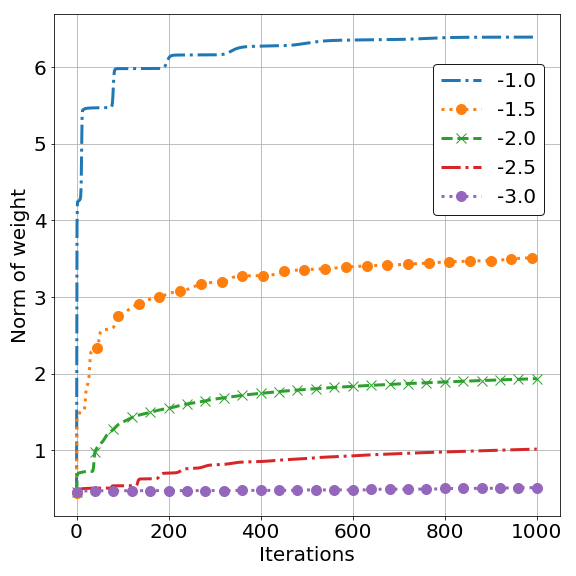
\includegraphics[width=0.5\textwidth]{figures/WN_direction.png}
\caption{Norm of parameters with different learning rate.}
\label{fig:weightnormgrowingnorm}
\end{figure}
}

\Answer{
${}$%placeholder
}
